\ifthenelse{\equal{\Langue}{FR}}{
\chapter{Hacheur 4 quadrants}
}{
\chapter{4 quadrants chopper}
}

\ifthenelse{\equal{\Langue}{FR}}{
Le schéma général du dispositif est celui de la figure suivante:
}{
The general scheme of the device is shown in the following figure:
}

\begin{figure}[h]
\centering

\includegraphics[width=\linewidth]{TP_H4Q/fig/TP_H4Q.png}
%\caption{Simplified internal control}
\end{figure}

\ifthenelse{\equal{\Langue}{FR}}{
L'alimentation $U_E$ est réalisée par un redressement triphasé du réseau 50 Hz variable jusqu'à 400 V au moyen d'un autotransformateur, suivi d'un condensateur de filtrage de valeur $C$. La machine à courant continu est à excitation indépendante qui sera maintenue constante avec un courant d'excitation égal à sa valeur nominale.

L'ensemble ``redresseur-hacheur'' est réalisé au sein d'un dispositif intégré SEMIKRON muni d'un système de commande externe permettant de réaliser une commande complémentaire synchrone ou décalée sur chacun des deux ``bras de pont''.

Le dispositif de commande permet de générer des signaux PWM dont le rapport cyclique peut être commandé à l'aide d'un potentiomètre ou une tension externe $v(t)$ \textbf{entre 0 et 5V}.
}{
The supply $U_E$ is provided by a three-phase rectification of the 50 Hz network, variable up to 400 V using an autotransformer, followed by a filtering capacitor of value $C$. The DC machine has independent excitation, which will be kept constant with an excitation current equal to its rated value.

The ``rectifier-chopper'' assembly is implemented within an integrated SEMIKRON device equipped with an external control system that allows for complementary synchronous or shifted control on each of the two ``bridge arms''.

The control device generates PWM signals whose duty cycle can be controlled using a potentiometer or an external voltage $v(t)$ \textbf{between 0 and 5V}.
}

\newpage
\ifthenelse{\equal{\Langue}{FR}}{
\section{Préparation}
}{
\section{Preparation}
}

\ifthenelse{\equal{\Langue}{FR}}{
On commande le hacheur avec les signaux de commande $f_1$, $f_2$, $f_3$ et $f_4$ ci-dessous. 
}{
The chopper is controlled with the control signals $f_1$, $f_2$, $f_3$ and $f_4$ below.
}

\begin{enumerate}
\ifthenelse{\equal{\Langue}{FR}}{
\item Tracer l'évolution de la tension de sortie du hacheur $U_m(t)$ en supposant que la tension d'entrée $U_e(t)$ est parfaitement constante.
\item Calculer la valeur moyenne de $U_m(t)$ en fonction de la tension d'entrée $U_e$ (supposée constante) et $\alpha$.
}{
\item Plot the evolution of the chopper output voltage $U_m(t)$ assuming that the input voltage $U_e(t)$ is perfectly constant.
\item Calculate the average value of $U_m(t)$ as a function of the input voltage $U_e$ (assumed constant) and $\alpha$.
}\end{enumerate}

\begin{figure}[h]
\centering
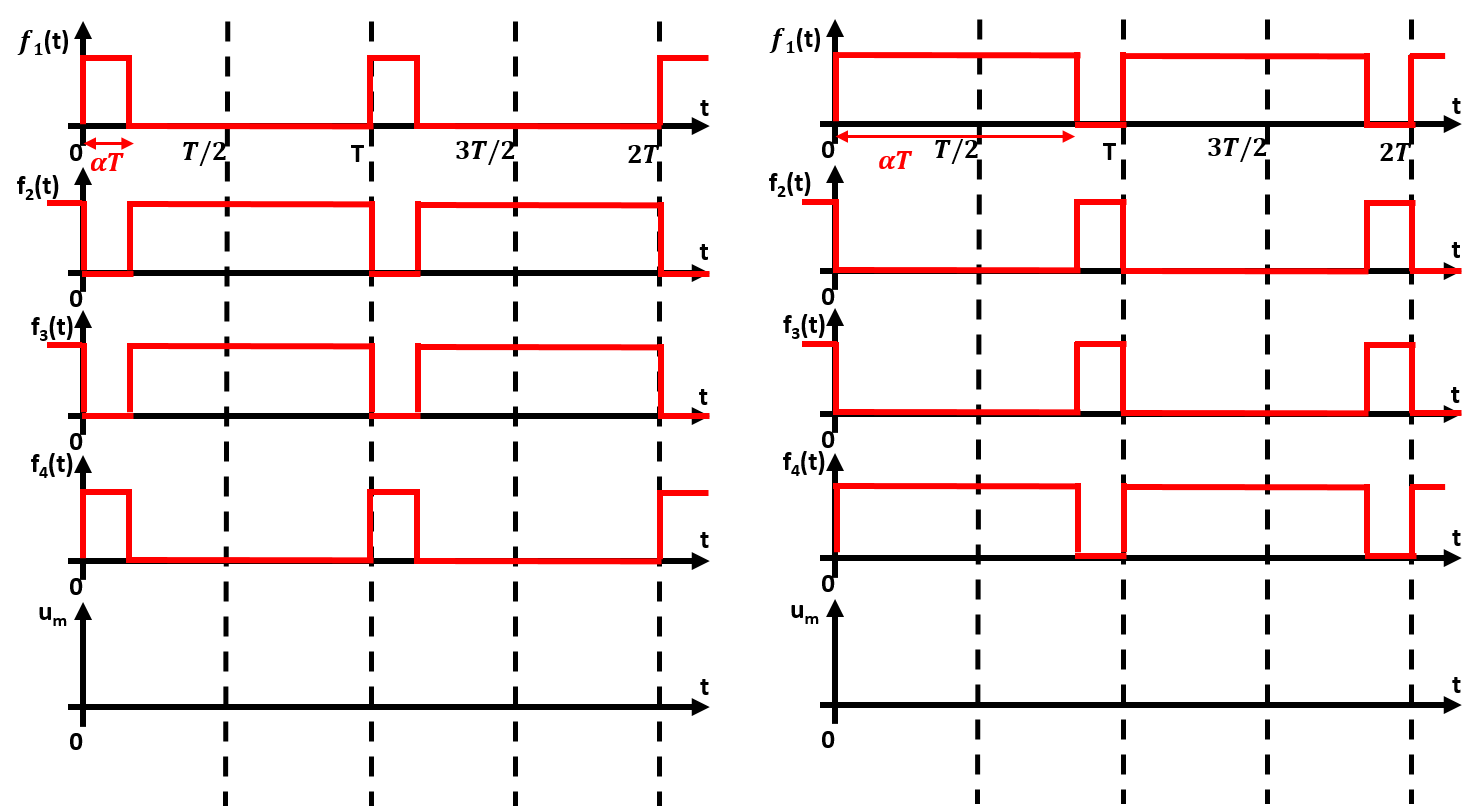
\includegraphics[width=1.1\linewidth]{TP_H4Q/fig/prepa_synchrone.png}
%\caption{Simplified internal control}
\end{figure}


\newpage
\ifthenelse{\equal{\Langue}{FR}}{
\section{Réalisation du montage}
}{
\section{Assembly of the circuit}
}

\begin{enumerate}
\ifthenelse{\equal{\Langue}{FR}}{
\item Relever les caractéristiques de la machine à courant continu et en déduire la valeur de la tension continue redressée $U_E$ nécessaire pour pouvoir exploiter toute la plage de vitesse de cette machine dans les deux sens. On majorera cette valeur ``théorique'' de $U_E$ de 20 \% pour tenir compte des chutes de tension et des limitations de rapport cycliques inhérentes à la boîte de commande.

\item Relever l'allure des signaux de commande notés $COM$ et $\overline{COM}$ sur la boîte de commande (on n'utilisera pas les signaux $DEC$ et $\overline{DEC}$). \textbf{On s'assurera que le rapport cyclique soit différent de 50 \%}. En déduire:
}{
\item Read the characteristics of the DC machine and deduce the value of the rectified DC voltage $U_E$ necessary to exploit the entire speed range of this machine in both directions. This ``theoretical'' value of $U_E$ will be increased by 20\% to take into account voltage drops and duty cycle limitations inherent to the control box.

\item Observe the shape of the control signals labeled $COM$ and $\overline{COM}$ on the control box (the signals $DEC$ and $\overline{DEC}$ will not be used). \textbf{Ensure that the duty cycle is different from 50\%}. Deduce:
}
\begin{itemize}
\ifthenelse{\equal{\Langue}{FR}}{
\item Le branchement des signaux de contrôle $COM$ et $\overline{COM}$
\item L'allure de la tension de sortie du hacheur, notamment son amplitude et sa fréquence.
}{
\item The connection of the control signals $COM$ and $\overline{COM}$
\item The shape of the chopper output voltage, particularly its amplitude and frequency.
}
\end{itemize}

\ifthenelse{\equal{\Langue}{FR}}{
\item Tracer la caractéristique de réglage de cette commande, i.e.\ le rapport cyclique de la commande $COM$ en fonction de la tension de commande externe (\textbf{variable dans l'intervalle 0 à 5V}). En déduire la valeur de cette tension imposant l'arrêt de la machine.

\item Réaliser le montage complet avec les recommandations suivantes:
}{
\item Plot the control characteristic of this command, i.e.\ the duty cycle of the $COM$ command as a function of the external control voltage (\textbf{variable in the range 0 to 5V}). Deduce the value of this voltage that imposes the stop of the machine.

\item Assemble the complete circuit with the following recommendations:
}
\begin{itemize}
\ifthenelse{\equal{\Langue}{FR}}{
\item laisser la machine à courant continu à vide;
\item si la machine est à excitation séparée, câbler en premier lieu son excitation et vérifier la valeur du courant correspondant;
\item régler la commande du hacheur pour imposer un rapport cyclique de 50\%;
\item augmenter progressivement la tension réseau (autotransformateur) jusqu'à atteindre la tension redressée $U_E$ souhaitée;
\item tester le bon fonctionnement du dispositif en faisant varier la commande du hacheur \textbf{lentement} dans les deux sens et en surveillant en permanence l'intensité du courant d'induit moteur.
}{
\item Leave the DC machine unloaded;
\item If the machine has separate excitation, first wire its excitation and check the corresponding current value;
\item Adjust the chopper control to impose a duty cycle of 50\%;
\item Gradually increase the network voltage (autotransformer) until the desired rectified voltage $U_E$ is reached;
\item Test the proper functioning of the device by varying the chopper control \textbf{slowly} in both directions while continuously monitoring the motor armature current.
}
\end{itemize}

\ifthenelse{\equal{\Langue}{FR}}{
Le montage étant assez ``volumineux'' à réaliser, il faudra prendre soin de câbler les différents blocs entre eux de manière aisément vérifiable. Les différents appareils de mesure devront être lisibles et l'oscilloscope sera aussi éloigné que possible des connexions de puissance.

\item Si le freinage du moteur est trop rapide, la tension de bus continu $U_E$ augmente. Pourquoi? \underline{\textbf{En présence de l'enseignant}}, observer ce phénomène.
}{
The assembly being quite ``bulky'' to implement, care should be taken to wire the different blocks together in a way that is easily verifiable. The various measuring devices should be readable, and the oscilloscope should be as far away as possible from the power connections.

\item If the motor braking is too fast, the DC bus voltage $U_E$ increases. Why? \newline\underline{\textbf{In the presence of the instructor}}, observe this phenomenon.
}
\end{enumerate}

\ifthenelse{\equal{\Langue}{FR}}{
\section{Caractérisation ``statique'' du dispositif}
}{
\section{Static Characteristics of the Device}
}

\begin{enumerate}[label={}]
\ifthenelse{\equal{\Langue}{FR}}{
\item \textbf{En vérifiant toujours que $U_E$ reste constante}, tracer la caractéristique du hacheur $<U_m>=f(\alpha)$, le moteur étant laissé à vide ($\alpha$ représente le rapport cyclique de la commande $COM$). Relever soigneusement les valeurs extrêmes de rapport cycliques possibles, $\alpha_{\min}$ et $\alpha_{\max}$.
}{
\item \textbf{Always ensuring that $U_E$ remains constant}, plot the chopper characteristic \newline$<U_m>=f(\alpha)$, with the motor left unloaded ($\alpha$ represents the duty cycle of the $COM$ command). Carefully record the extreme values of possible duty cycles, $\alpha_{\min}$ and $\alpha_{\max}$.
}
\end{enumerate}

\ifthenelse{\equal{\Langue}{FR}}{
\section{Etude du hacheur en régime dynamique}
}{
\section{Study of the Chopper in Dynamic Regime}
}

\ifthenelse{\equal{\Langue}{FR}}{
Dans cette étude, il faut générer un rapport cyclique du type: $\alpha(t) = \alpha_0 + \Delta\alpha(t)$ où $\Delta\alpha(t)$ est une variation ``lente'' et $\alpha_0 = 0.5$. Pour cela, la tension de commande utilisée pour piloter le dispositif comprend une composante continue $v_0$ et une composante alternative de fréquence faible, notée $\Delta v(t)$. On laissera toujours le moteur à vide \textbf{et l'on prendra soin de ne pas commuter les fonctions du générateur de commande avec un montage sous tension} afin d'éviter les surintensités.
}{
In this study, a duty cycle of the type $\alpha(t) = \alpha_0 + \Delta\alpha(t)$ must be generated, where $\Delta\alpha(t)$ is a ``slow'' variation and $\alpha_0 = 0.5$. To achieve this, the control voltage used to drive the device includes a DC component $v_0$ and a low-frequency AC component, denoted $\Delta v(t)$. The motor will always be left unloaded \textbf{and care will be taken not to switch the functions of the control generator with a powered circuit} to avoid overcurrents.
}

\begin{enumerate}
\ifthenelse{\equal{\Langue}{FR}}{
\item Utiliser la caractéristique de réglage précédente pour déterminer $v_0$ et $\Delta v(t)$ afin de faire varier le rapport cyclique linéairement entre 0.3 et 0.7. Appliquer cette tension progressivement sur le dispositif (amplitude lentement augmentée), à une fréquence de 0.3 Hz environ (fréquence du signal $\Delta v$).

\item Relever alors simultanément le courant d'induit moteur $i_M$ et la tension mesurée par la génératrice tachymétrique $v_T$ (image de la vitesse $\Omega$). Comment interpréter ces courbes en utilisant le mode XY de l'oscilloscope (avec une rémanence suffisante)? On pourra améliorer la mesure en intercalant un filtre passe bas sur la mesure du courant afin d'éliminer son ondulation. Comment choisir la fréquence de coupure de ce filtre?

\item Observer simultanément la vitesse, le courant d'induit et la tension d'entrée $U_e(t)$. Expliquer les variations observées sur $U_e(t)$ et lier celles-ci aux 4 quadrants de fonctionnement.
}{
\item Use the previous control characteristic to determine $v_0$ and $\Delta v(t)$ in order to linearly vary the duty cycle between 0.3 and 0.7. Apply this voltage gradually to the device (slowly increasing amplitude), at a cycle frequency of 0.3 Hz (frequency of the $\Delta v$ signal).

\item Simultaneously record the motor armature current $i_M$ and the voltage measured by the tachogenerator $v_T$ (image of the speed $\Omega$). How to interpret these curves using the XY mode of the oscilloscope (with sufficient persistence)? The measurement can be improved by inserting a low-pass filter on the current measurement to eliminate its ripple. How to choose the cutoff frequency of this filter?
}
\end{enumerate}

\ifthenelse{\equal{\Langue}{FR}}{
\section{Pour aller plus loin: Onduleur}
}{
\section{To go further: Inverter}
}

\ifthenelse{\equal{\Langue}{FR}}{
Remplacer le moteur par une charge R-L série. On souhaite alimenter cette charge avec le réseau électrique nord-américain (110V / 60 Hz) à partir de notre réseau (230V / 50 Hz). On va donc utiliser le hacheur en ``onduleur'' monophasé afin de récréer ce réseau. Pour cela, on utilisera un rapport cyclique de la forme $\alpha(t) = \alpha_0 + \delta\alpha. \sin(\omega t)$
}{
Replace the motor with a series R-L load. We want to power this load with the North American power grid (110V / 60 Hz) from our power grid (230V / 50 Hz). We will therefore use the chopper as a single-phase ``inverter'' to recreate this network. For this, we will use a duty cycle of the form $\alpha(t) = \alpha_0 + \delta\alpha. \sin(\omega t)$.
}
\begin{enumerate}
\ifthenelse{\equal{\Langue}{FR}}{
\item Déterminer $\alpha_0$, $\delta\alpha$ et $\omega$ afin de recréer le réseau désiré.

\item Appliquer cette commande et alimenter la charge. Observer la tension $U_m$ en sortie du hacheur et $U_r$ la tension aux bornes de la résistance.
}{
\item Determine $\alpha_0$, $\delta\alpha$ and $\omega$ in order to recreate the desired power grid.

\item Apply this command and power the load. Observe the voltage $U_m$ at the chopper output and $U_r$ the voltage across the resistor.
}
\end{enumerate}



